%%%%%%%% Sample LaTeX input for Complex Systems %%%%%%%%%%% 
% Revision 4, Jun 27, 2018
%
% This is a LaTeX input file  
% Text following % on a particular line is treated as a comment, and 
% ignored by LaTeX.  
% You do not need to type any text that follows a % 
% 
\documentclass{article}

\usepackage{graphicx,hyperref}
\usepackage{amssymb,ComplexSystems}
\usepackage{tikz}
\usepackage{scalefnt}

\usetikzlibrary{automata, positioning, arrows}
\usepackage{underscore}
\graphicspath{ {./images/} }

\usepackage{listings}
\usepackage{color}

\definecolor{dkgreen}{rgb}{0,0.6,0}
\definecolor{gray}{rgb}{0.5,0.5,0.5}
\definecolor{mauve}{rgb}{0.58,0,0.82}

\lstset{frame=tb,
  language=Java,
  aboveskip=3mm,
  belowskip=3mm,
  showstringspaces=false,
  columns=flexible,
  basicstyle={\small\ttfamily},
  numbers=none,
  numberstyle=\tiny\color{gray},
  keywordstyle=\color{blue},
  commentstyle=\color{dkgreen},
  stringstyle=\color{mauve},
  breaklines=true,
  breakatwhitespace=true,
  tabsize=3
}

% complex-systems.sty is the macro package for Complex Systems.
% It is available at
% http://www.complex-systems.com/samples/complex-systems.sty
% epsf.sty is the preferred graphics import method
\makeindex

\begin{document}

\title{Documentation - Data Bases 2%
% Use \\ to indicate line breaks in titles longer than about 
% 55 characters. 
%
}

\author{\authname{Marco Fasanella}\\[2pt] 
% Use \\[2pt] to end the line and add space between author name and affiliation. 
\authadd{MsC Computer Science, Polimi}\\
\authadd{C.P. 10617541}\\
\and
% For extra space, precede the second set of authors with \and.
\authname{Nicola Dean}\\
\authadd{MsC Computer Science, Polimi}\\
\authadd{C.P. 10674826}\\
% Do not use a ``.'' at the end of any line in the address. 
}

% The following specifies the running headings 
%
% Each running heading should be less than about 50 characters long. 
% If necessary, give a shortened version of the title. 
%
% Use initials for first and second names. If all author names do not fit, truncate the 
% list and end with ``et al.''.
\markboth{Data Base 2 Project} 
{Design Documentation}

\maketitle
% End title section

\begin{abstract}
This document describes design and implementation of Data Base 2 Project
\end{abstract}

% The text of the paper follows. All of the text should be in the same file. 
% Use separate files for large tabular material and graphics.
%\printindex
\section{Specifications}
\label{intro}
% \label is a hyperlink target for cross-referencing to this section using \ref{intro} (optional).
A telco company offers pre-paid online services to web users. Two client applications using the same database have been developed: a costumer application and an employee application.
\subsection{Extra hypotesis}

\section{ER Diagram}

\begin{figure}[hbt!]
\centering
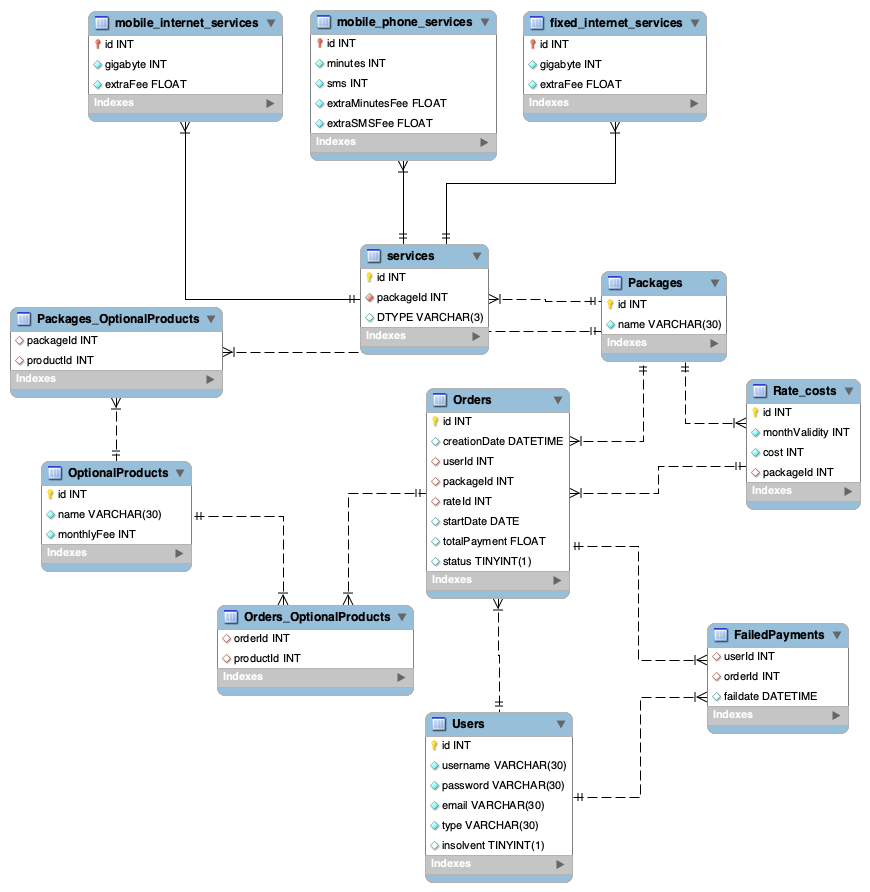
\includegraphics[width=0.86\textwidth]{er.png}
\caption{ER Diagram}
\end{figure}



\section{SQL Description}
Detailed description of SQL code used in the project.

\subsection{Views}
The following views are used for various Sales Reports.



Joining Orders and Rate_costs tables we performed a \emph{selection} for each distinct package (depending on their month validity) and a \emph{count} for their occurrences.
\begin{verbatim}
create view PurchasesCount as (
       Select Packages.name as name,Rate_costs.monthValidity as validity, count(*) as count
       from Orders as o join Packages  join Rate_costs
       on o.packageId=Packages.id and Rate_costs.packageId=o.packageId 
       and o.rateId=Rate_costs.id
       group by o.packageId, Rate_costs.id
           );
\end{verbatim}
Then for a less detailed view, from \emph{PurchasesCount} , a \emph{group by} on the name of the package gives a count of each one.
\begin{verbatim}
create view PurchasesCountGrouped as (
       select p.name as name, sum(p.count) as count
       from PurchasesCount as p
       group by p.name
           );

\end{verbatim}

To count the Optional Products was necessary a \emph{left join} because it could exist a Package without any Optional Product, and as a consequence it wouldn't be stored in \emph{Orders_OptionalProducts} table.
\begin{verbatim}
create view OptionalProductsCount as(
       select o.packageId as packageId, count(opt.productId) as optcount
       from Orders as o left join Orders_OptionalProducts as opt
       on o.id=opt.orderId
       group by o.id
           );
\end{verbatim}
Then to have the average count of them, we performed an \emph{avg} on the count of previous view.
\begin{verbatim}
create view OptionalProductsAverage as(
       select p.name as name, avg(opc.optcount) as avg
       from OptionalProductsCount as opc join Packages as p
       where opc.packageId=p.id
       group by id
           );
           
\end{verbatim}

Following view sums the \emph{totalPayment} of each Order grouped by \emph{packageId}
\begin{verbatim}
create view ValueOfTotalSales as(
       select p.name as name, sum(o.totalPayment) as totalPayment
       from Orders as o join Packages as p
       where p.id=o.packageId
       group by o.packageId
           );
\end{verbatim}
Then in \emph{OptionalProductsSales} the same method is used to get the totalCost of the Optional Products related to their corresponding Service Package in \emph{Orderds}
\begin{verbatim}
create view OptionalProductsSales as(
     select p.name as name,sum(op.monthlyFee*r.monthValidity) as totalOptionalProductsSales
     from Orders_OptionalProducts as orderop join Orders as o
     join OptionalProducts as op join Packages as p join Rate_costs as r
     where o.id=orderop.orderId and orderop.productId=op.id 
     and o.packageId=p.id and o.rateId=r.id
     group by p.id
          );
\end{verbatim}

And finally these two views are \emph{left joined} to have both \emph{totalPayment} with and without Optional Products. A \emph{left join} is required because as mentioned before it could exist a service package without Optional Product. In this case \emph{totalPaymentWithoutOP} will return \emph{null}.
\begin{verbatim}
create view ValueOfSalesDetailed as(
       select vot.name as name, vot.totalPayment as totalPayment, 
               (vot.totalPayment-ops.totalOptionalProductsSales) as totalPaymentWithoutOP
       from ValueOfTotalSales as vot left join OptionalProductsSales as ops
       on vot.name=ops.name
         );
\end{verbatim}                                     


In \emph{InsolventReport} are selected all Users with \emph{having count(*)>=3} of insolvent orders stored in \emph{FailedPayments}.
\begin{verbatim}
create view InsolventReport as(
        select u.id as id,u.username as username,u.email as email,
              (
              select max(fp1.faildate) 
              from FailedPayments as fp1  
              where fp1.userId=u.id) as lastDate,
              (
              select o.totalPayment 
              from Orders as o join FailedPayments as fp2 
              where o.id=fp2.orderId and lastdate=fp2.faildate) as amount
        from FailedPayments as fp join Users as u
        where fp.userId=u.id
        group by u.id
        having count(*)>=3
           );
\end{verbatim}

Last view  \emph{OptionalProductBestSeller} is used to have a count and the value of total sales of each Optional Product.
\begin{verbatim}
create view OptionalProductBestSeller as(
        select op.name as name,count(op.id) as amountSold, 
               sum(op.monthlyFee*r.monthValidity) as value
        from Orders_OptionalProducts as ordop join OptionalProducts as op 
        join Rate_costs as r join Orders as o
        where ordop.productId=op.id and o.rateId=r.id and o.id=ordop.orderId
        group by op.id
             );
\end{verbatim}
The using two distinct queries we performed the  \emph{OptionalProductBestSellerForValue}
\begin{verbatim}
        select o 
        from OptionalProductBestSeller o 
        where o.value=(
        select max(o2.value) 
        from OptionalProductBestSeller o2
        );
\end{verbatim}
and  \emph{OptionalProductBestSellerForAmount}
\begin{verbatim}
          select o from OptionalProductBestSeller o 
          where o.amountSold=(
          select max(o2.amountSold) 
          from OptionalProductBestSeller o2
          );
\end{verbatim}

\subsection{Triggers}
\begin{verbatim}
create trigger INSOLVENT_USER
    after insert on Orders
    for each row
begin
    if ( new.status = false) then
    update Users set Users.insolvent = true where Users.id = new.userId;
    insert into FailedPayments (userId,orderId,faildate) 
    values (new.userId,new.id,CURRENT_TIMESTAMP);
end if;
\end{verbatim}



\begin{verbatim}
create trigger INSOLVENT_USER_REMOVAL
    after update on Orders
    for each row
begin
    if (new.status = true) AND
		     (select count(*) from Orders as o where o.userId=new.userId and o.status = false) = 0
		then
    update Users set Users.insolvent = false where Users.id = new.userId;
end if;
if (new.status = false AND old.status = new.status)  then
			insert into FailedPayments (userId,orderId,faildate) 
			values (new.userId,new.id,CURRENT_TIMESTAMP);
end if;
\end{verbatim}

\section{ORM Description}

\subsection{Entities}

\paragraph{Optional Product}

\begin{lstlisting}
@Entity
@Table(name = "OptionalProducts", schema = "test")
public class OptionalProduct{

    @Id
    @GeneratedValue(strategy= GenerationType.IDENTITY)
    int     id;
    String  name;
    int     monthlyFee;
\end{lstlisting}

\paragraph{Order}
The Order entity refers to Table \emph{Orders}
\begin{lstlisting}
@Entity
@Table(name = "Orders", schema = "test")
@NamedQuery(name="Orders.Id" ,  query="select o from Order o where o.Id = :orderId")
@NamedQuery(name="Orders.All" , query="select o from Order o") @NamedQuery(name="Orders.Suspended" , query="select o from Order o where o.status=false")
@NamedQuery(name="Orders.RemoveSuspend" , query="update Order o set o.status = true where o.Id=:orderId")
@NamedQuery(name="PurchasesByPackages" , query = "select count (distinct o) from Order o group by o.pack")
@NamedQuery(name="PurchasesByPackagesID" , query = "select  o.pack.name, count(o.pack) from Order o where o.status=true group by o.pack ")
@NamedQuery(name="Orders.UserInsolvances" , query = "select o from Order o where o.status=false and o.user.id = :userId")

public class Order {

    @Id
    @GeneratedValue(strategy= GenerationType.IDENTITY)
    int Id;
    Date startDate;
    Date creationDate;
    float totalPayment;
    Boolean status =null;
    
\end{lstlisting}


\paragraph{RateCost}

\begin{lstlisting}
@Entity
@Table(name="Rate_costs", schema = "test")
public class RateCost {

    @Id
    @GeneratedValue(strategy= GenerationType.IDENTITY)
    int id;
    int monthValidity;
    int cost;
    int packageId;
\end{lstlisting}

\paragraph{Service}
\begin{lstlisting}
@Entity
@Inheritance(strategy = InheritanceType.JOINED)
@Table(name = "services", schema = "test")
public class Service {
    @Id
    @GeneratedValue(strategy=GenerationType.IDENTITY)
    int id;
    int packageId;
    @Column(name = "DTYPE")
    String type;
\end{lstlisting}

\paragraph{User}
\begin{lstlisting}
@Entity
@NamedQuery(name = "User.authentication", query = "select usr from User usr WHERE usr.username = :username and usr.password = :password")
@NamedQuery(name = "User.insolvent"     , query = "select usr from User usr WHERE usr.insolvent = true")
@Table(name="Users", schema = "test")
public class User {
    @Id
    @GeneratedValue(strategy=GenerationType.IDENTITY)
    int id;

    String  username;
    String  password;
    String  email;
    String  type;
    boolean insolvent;
\end{lstlisting}

\begin{lstlisting}

\end{lstlisting}


\section{Application Components}
\section{UML sequence diagrams}

\end{document}